
\section{要求補正情報}
% TODO: 3.要求仕様ではなく要求補正情報の方がよさそう.要求仕様にするなら,柔軟性をもたせる設計にするとか書く必要がありそう.

PDRと他の情報を使ってライブラリを作成する上で,
どのような状況や環境が存在し補正に利用できるのかその具体的な例を考える必要がある.
例えば大学内や病院などのWi-FiのAPが多く設置されている場所では,
Wi-Fiの電波強度を利用した位置推定が有効である.
他の例として展示会場や大きなアトリウムなどの広い開放空間が考えられる.
このような場所ではWi-FiのAPの配置が難しく,
信号のカバレッジが不均一になりやすくWi-Fiを利用した位置推定は難しい.
このような場所の場合BLEビーコンを配置してその電波強度を利用した位置推定が有効である.
また2章で示したように\cite{pdr-wifi}\cite{pdr-ble}などのPDRと電波を利用した推定に関する研究は盛んに行われている.
このように電波を使った手法は多くの場所で有効であり,補正に利用可能な情報として重要度が高い.
そのため本ライブラリにおいても採用を行う.
他に補正に利用可能な情報としてフロアマップ情報がある.
フロアマップ情報は多くの場所で比較的入手が容易だと思われる.
そのため本ライブラリにおいても採用を行う.

磁気やカメラなどの情報は,磁気はデータが繊細であり電波と比べると補正に利用する難易度が高い,
カメラはプライバシーなどの問題があり本ライブラリの基礎段階においてこれらを採用しない.
また気圧センサは基礎段階として3次元空間を推定対象としないため採用しない.


\begin{figure}[ht]
	\centering
	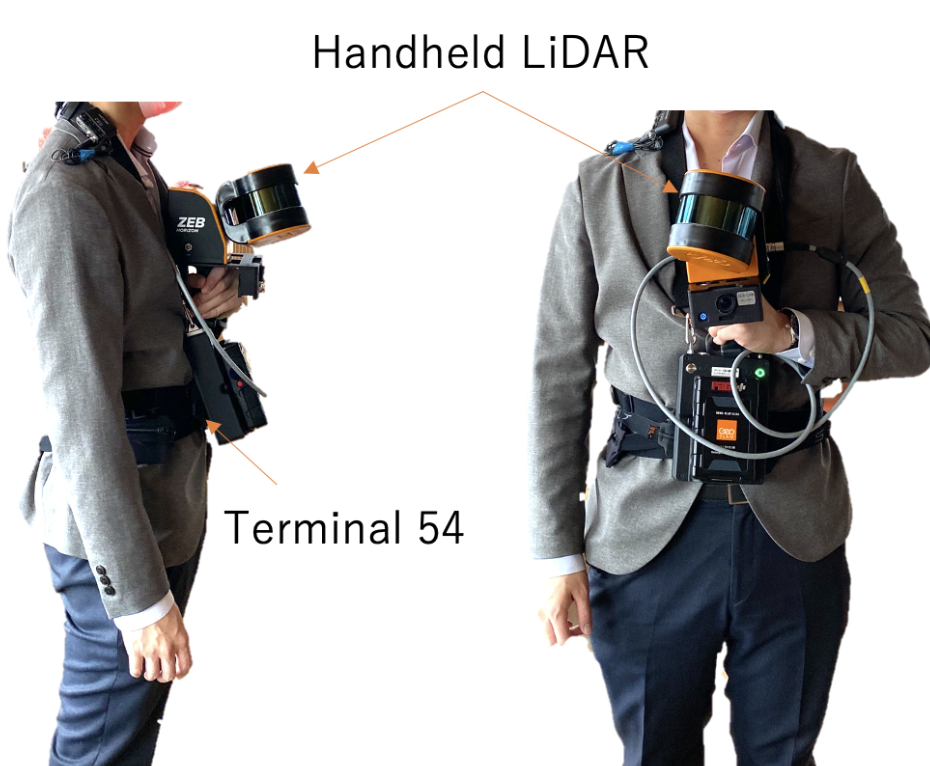
\includegraphics[width=\linewidth]{image/lidar.jpg}
	\caption{歩行者の装着器具}    \label{fig:step_detect}
\end{figure}




